\documentclass[a4paper]{article}
\usepackage[italian]{babel}
\usepackage[left=1cm, right=1cm, bottom=2cm, top=2cm]{geometry}
\usepackage{csvsimple}
\usepackage[utf8]{inputenc}
\usepackage{float}
\usepackage[table,xcdraw]{xcolor}
\usepackage[scaled]{helvet}
\renewcommand\familydefault{\sfdefault} 
\usepackage{pgfplots}
\usepackage{multirow}
\usepackage[table,xcdraw]{xcolor}
\pgfplotsset{compat=newest}
\usepackage{pdflscape}
%opening
\title{Relazione laboratorio Algoritmi Avanzati}
\author{Magarotto Francesco\\Muraro Enrico\\Piva Giulio}

\begin{document}
\rowcolors{2}{gray!25}{white}
\begin{titlepage}
  \vspace*{5cm}
  \begin{center}
    \Large\bfseries
    Relazione di laboratorio
  \end{center}
  \begin{center}
    \large
    Corso di Algoritmi Avanzati\\
    Laurea Magistrale in Informatica\\A.A. 2019-2020
  \end{center}
  \vspace{4cm plus 1fill}
  \begin{flushleft}
    \large
    Magarotto Francesco - 1236594\\Muraro Enrico - 1238899 \\Piva Giulio - 1242455
  \end{flushleft}
\end{titlepage}
\newpage


\newpage

%\begin{figure}[H]
%\centering
%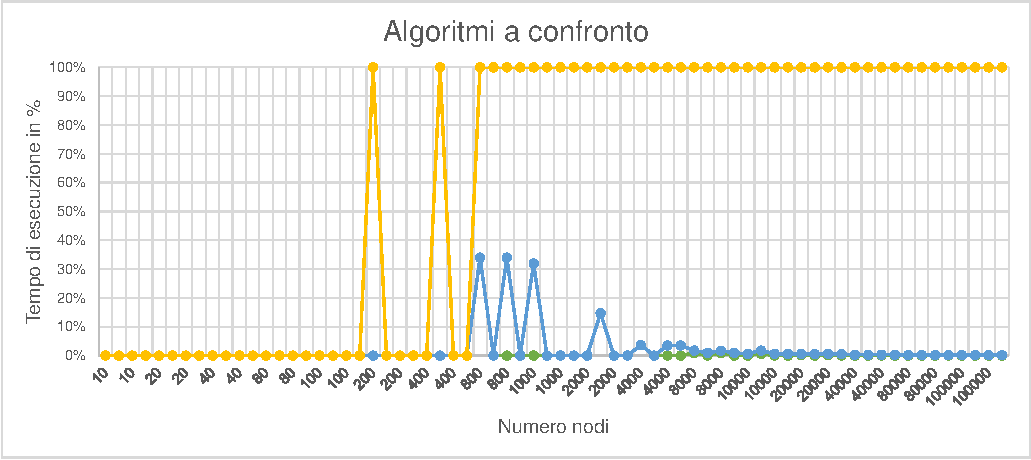
\includegraphics[scale=1]{grafici/confronto.pdf}
%\caption{Grafico che mette in relazione i tempi di esecuzione dei tre algoritmi in base al tempo richiesto per la loro esecuzione}
%\end{figure}
\begin{landscape}
\section{Risultati ottenuti}
% Please add the following required packages to your document preamble:
% \usepackage{multirow}
% \usepackage[table,xcdraw]{xcolor}
% If you use beamer only pass "xcolor=table" option, i.e. \documentclass[xcolor=table]{beamer}
\begin{table}[H]
\begin{tabular}{|l|l|l|l|l|l|l|l|l|l|}
\hline
\rowcolor[HTML]{FFFFFF} 
\multicolumn{1}{|c|}{\cellcolor[HTML]{FFFFFF}{\color[HTML]{000000} }}                                   & \multicolumn{3}{c|}{\cellcolor[HTML]{FFFFFF}{\color[HTML]{000000} \textbf{Held-Karp}}}                                                     & \multicolumn{3}{c|}{\cellcolor[HTML]{FFFFFF}{\color[HTML]{000000} \textbf{Nearest Approx}}}                                                & \multicolumn{3}{c|}{\cellcolor[HTML]{FFFFFF}{\color[HTML]{000000} \textbf{2 Approx}}}                                                      \\ \cline{2-10} 
\rowcolor[HTML]{FFFFFF} 
\multicolumn{1}{|c|}{\multirow{-2}{*}{\cellcolor[HTML]{FFFFFF}{\color[HTML]{000000} \textbf{Istanza}}}} & {\color[HTML]{000000} \textbf{Soluzione ottima}} & {\color[HTML]{000000} \textbf{Tempo (s)}} & {\color[HTML]{000000} \textbf{Errore (\%)}} & {\color[HTML]{000000} \textbf{Soluzione ottima}} & {\color[HTML]{000000} \textbf{Tempo (s)}} & {\color[HTML]{000000} \textbf{Errore (\%)}} & {\color[HTML]{000000} \textbf{Soluzione ottima}} & {\color[HTML]{000000} \textbf{Tempo (s)}} & {\color[HTML]{000000} \textbf{Errore (\%)}} \\ \hline
{\color[HTML]{000000} berlin52.tsp}                                                                     & {\color[HTML]{000000} 18891,00}                  & {\color[HTML]{000000} 120004}             & {\color[HTML]{000000} 150\%}                & {\color[HTML]{000000} 8962}                      & {\color[HTML]{000000} 1}                  & {\color[HTML]{000000} 19\%}                 & {\color[HTML]{000000} 10386}                     & {\color[HTML]{000000} 3}                  & {\color[HTML]{000000} 38\%}                 \\ \hline
\rowcolor[HTML]{EFEFEF} 
{\color[HTML]{000000} burma14.tsp}                                                                      & {\color[HTML]{000000} 3323,00}                   & {\color[HTML]{000000} 912}                & {\color[HTML]{000000} 0\%}                  & {\color[HTML]{000000} 4048}                      & {\color[HTML]{000000} 0}                  & {\color[HTML]{000000} 22\%}                 & {\color[HTML]{000000} 4003}                      & {\color[HTML]{000000} 0}                  & {\color[HTML]{000000} 20\%}                 \\ \hline
{\color[HTML]{000000} ch150.tsp}                                                                        & {\color[HTML]{000000} 48265,00}                  & {\color[HTML]{000000} 120002}             & {\color[HTML]{000000} 639\%}                & {\color[HTML]{000000} 7784}                      & {\color[HTML]{000000} 1}                  & {\color[HTML]{000000} 19\%}                 & {\color[HTML]{000000} 8914}                      & {\color[HTML]{000000} 6}                  & {\color[HTML]{000000} 37\%}                 \\ \hline
\rowcolor[HTML]{EFEFEF} 
{\color[HTML]{000000} d493.tsp}                                                                         & {\color[HTML]{000000} 112695,00}                 & {\color[HTML]{000000} 120002}             & {\color[HTML]{000000} 222\%}                & {\color[HTML]{000000} 43713}                     & {\color[HTML]{000000} 8}                  & {\color[HTML]{000000} 25\%}                 & {\color[HTML]{000000} 45450}                     & {\color[HTML]{000000} 28}                 & {\color[HTML]{000000} 30\%}                 \\ \hline
{\color[HTML]{000000} dsj1000.tsp}                                                                      & {\color[HTML]{000000} 5,52E+16}                  & {\color[HTML]{000000} 120007}             & {\color[HTML]{000000} 2861\%}               & {\color[HTML]{000000} 24630468}                  & {\color[HTML]{000000} 6}                  & {\color[HTML]{000000} 32\%}                 & {\color[HTML]{000000} 25525517}                  & {\color[HTML]{000000} 0,03}               & {\color[HTML]{000000} 37\%}                 \\ \hline
\rowcolor[HTML]{EFEFEF} 
{\color[HTML]{000000} eil51.tsp}                                                                        & {\color[HTML]{000000} 1063,00}                   & {\color[HTML]{000000} 120001}             & {\color[HTML]{000000} 150\%}                & {\color[HTML]{000000} 512}                       & {\color[HTML]{000000} 0}                  & {\color[HTML]{000000} 20\%}                 & {\color[HTML]{000000} 591}                       & {\color[HTML]{000000} 0}                  & {\color[HTML]{000000} 39\%}                 \\ \hline
{\color[HTML]{000000} gr202.tsp}                                                                        & {\color[HTML]{000000} 72929,00}                  & {\color[HTML]{000000} 120004}             & {\color[HTML]{000000} 82\%}                 & {\color[HTML]{000000} 49899}                     & {\color[HTML]{000000} 0}                  & {\color[HTML]{000000} 24\%}                 & {\color[HTML]{000000} 52615}                     & {\color[HTML]{000000} 3}                  & {\color[HTML]{000000} 31\%}                 \\ \hline
\rowcolor[HTML]{EFEFEF} 
{\color[HTML]{000000} gr229.tsp}                                                                        & {\color[HTML]{000000} 182845,00}                 & {\color[HTML]{000000} 120001}             & {\color[HTML]{000000} 36\%}                 & {\color[HTML]{000000} 162430}                    & {\color[HTML]{000000} 1}                  & {\color[HTML]{000000} 21\%}                 & {\color[HTML]{000000} 179335}                    & {\color[HTML]{000000} 2}                  & {\color[HTML]{000000} 33\%}                 \\ \hline
{\color[HTML]{000000} kroA100.tsp}                                                                      & {\color[HTML]{000000} 172822,00}                 & {\color[HTML]{000000} 120001}             & {\color[HTML]{000000} 712\%}                & {\color[HTML]{000000} 26991}                     & {\color[HTML]{000000} 0}                  & {\color[HTML]{000000} 27\%}                 & {\color[HTML]{000000} 30472}                     & {\color[HTML]{000000} 1}                  & {\color[HTML]{000000} 43\%}                 \\ \hline
\rowcolor[HTML]{EFEFEF} 
{\color[HTML]{000000} kroD100.tsp}                                                                      & {\color[HTML]{000000} 148492,00}                 & {\color[HTML]{000000} 120001}             & {\color[HTML]{000000} 597\%}                & {\color[HTML]{000000} 26906}                     & {\color[HTML]{000000} 0}                  & {\color[HTML]{000000} 26\%}                 & {\color[HTML]{000000} 28553}                     & {\color[HTML]{000000} 1}                  & {\color[HTML]{000000} 34\%}                 \\ \hline
{\color[HTML]{000000} pcb442.tsp}                                                                       & {\color[HTML]{000000} 229554,00}                 & {\color[HTML]{000000} 120002}             & {\color[HTML]{000000} 352\%}                & {\color[HTML]{000000} 61551}                     & {\color[HTML]{000000} 1}                  & {\color[HTML]{000000} 21\%}                 & {\color[HTML]{000000} 73876}                     & {\color[HTML]{000000} 7}                  & {\color[HTML]{000000} 45\%}                 \\ \hline
\rowcolor[HTML]{EFEFEF} 
{\color[HTML]{000000} ulysses16.tsp}                                                                    & {\color[HTML]{000000} 6859,00}                   & {\color[HTML]{000000} 16289}              & {\color[HTML]{000000} 0\%}                  & {\color[HTML]{000000} 9988}                      & {\color[HTML]{000000} 0}                  & {\color[HTML]{000000} 46\%}                 & {\color[HTML]{000000} 7788}                      & {\color[HTML]{000000} 0}                  & {\color[HTML]{000000} 14\%}                 \\ \hline
{\color[HTML]{000000} ulysses22.tsp}                                                                    & {\color[HTML]{000000} 8649,00}                   & {\color[HTML]{000000} 120002}             & {\color[HTML]{000000} 23\%}                 & {\color[HTML]{000000} 10586}                     & {\color[HTML]{000000} 0}                  & {\color[HTML]{000000} 51\%}                 & {\color[HTML]{000000} 8308}                      & {\color[HTML]{000000} 0}                  & {\color[HTML]{000000} 18\%}                 \\ \hline
\end{tabular}
\end{table}
\end{landscape}

\end{document}
